\subsection{Steeringklassen} \label{sec:steering_impl}

Steering klassen er den klasse der kontrollere PWM signalet til motorens fremdrift og til styretøj servoen. 
Den modtager nye input fra systemet om ændringer af fremdrift, brems og retning på styretøj. Derudover henter den, hver gang klassen skal opdaterer PWM signalet til motoren, den aktuelle hastighed på bilen fra Dataklassen. 
Klassen har kun en public metode som kan kaldes, \texttt{userInput()}. I listing \ref{lst:steering_header} ses implementering af klassens headerfilen.

\lstinputlisting[linerange=Steering::header1-Steering::header2, label=lst:steering_header, caption=\texttt{Header} for Steeringklassen.]{../../src/bil/steering/steering.hpp}

Constructoren sørger primært for at sætte WiringPi op. Se sektion \ref{sec:wiringPi_impl}. 
Der er en HW og SW PWM del der skal initialiseres. 
Udover opsætning starter den en separat tråd der kører \texttt{PWMUpdate} i et loop indtil systemet lukkes ned. 
Samt at sætte værdier for PID regulering af motoren 

\lstinputlisting[linerange=Steering::Steering1-Steering::Steering2, label=lst:steering_con, caption=\texttt{Constructor} for Steeringklassen.]{../../src/bil/steering/steering.cpp}


Deconstructoren sørger for at lukke \texttt{Steering::PWMUpdate} tråden ned og joine med den, slukke for HW og SW PWM og digitale outputs til styring af H-broen.

\lstinputlisting[linerange=Steering::~Steering1-Steering::~Steering2, label=lst:steering_decon, caption=\texttt{Deconstructor} for Steeringklassen.]{../../src/bil/steering/steering.cpp}

Metoden \texttt{userInput} er den eneste metode der kan tilgås udefra. Den håndtere værdier fra Xbox 360 kontrolleren. Den omregner frem og tilbage værdierne i forhold den max hastighed der er sat for bilen. Max hastigheden hentes fra Settings klassen. Hvis der skal bremses går den direkte til \texttt{brake} metoden. Tilsidst kalder \texttt{turn} metoden

\lstinputlisting[linerange=Steering::userInput1-Steering::userInput2, label=lst:steering_userInput, caption=Metoden \texttt{userInput} Steeringklassen.]{../../src/bil/steering/steering.cpp} 

\texttt{brake} metoden bremser bilen ved at sætte motor PWM til 100 \% og de 2 retnings digitale outputs lave. Det får H-broen til at bremse motoren aktivt. Mens der bremses bliver PWM i \texttt{PWMUpdate} ikke opdateret.
\lstinputlisting[linerange=Steering::brake1-Steering::brake2, label=lst:steering_brake, caption=Metoden \texttt{brake} Steeringklassen.]{../../src/bil/steering/steering.cpp}

\texttt{softbrake} metoden sætte motor PWM til 0 \% og de 2 retnings digitale outputs lave. 
Derved vil bilen begynde at løbe farten af.
\lstinputlisting[linerange=Steering::softbrake1-Steering::softbrake2, label=lst:steering_softbrake, caption=Metoden \texttt{softbrake} Steeringklassen.]{../../src/bil/steering/steering.cpp}

\texttt{turn} metoden omregner styre værdierne fra Xbox kontrolleren til en duty cycle for SW PWM mellem 0,5ms og 2.5ms. 
Som vil give max udslag til begge sider. 
\lstinputlisting[linerange=Steering::turn1-Steering::turn2, label=lst:steering_turn, caption=Metoden \texttt{turn} Steeringklassen.]{../../src/bil/steering/steering.cpp}

\texttt{motorSetPWM} metoden bestemmer om bilen skal sættes til at kører frem eller tilbage ud fra den aktuelle retning og input fra Xbox kontrolleren. 
Hvis det er nødvendig at kører den modsatte vej bremses der indtil den er under en vis hastighed
. 
\lstinputlisting[linerange=Steering::motorSetPWM1-Steering::motorSetPWM2, label=lst:steering_motorSetPWM, caption=Metoden \texttt{motorSetPWM} Steeringklassen.]{../../src/bil/steering/steering.cpp}

\texttt{PWMUpdate} metoden kører i sin egen tråd. Den henter hver gang den aktuelle hastighed på bilen fra \texttt{Dataklassen} og udregner fejlen i forhold til den ønskede hastighed. Herefter udregner værdierne for PID reguleringen. Og til sidst sættes den nye PWM værdi på motoren. 
\lstinputlisting[linerange=Steering::PWMUpdate1-Steering::PWMUpdate2, label=lst:steering_PWMUpdate, caption=Metoden \texttt{PWMUpdate} Steeringklassen.]{../../src/bil/steering/steering.cpp}

\subsubsection{Test af Steering klassen}

For at test Steering klassen blev det skrevet et lille test program. Det kan ses i listings \ref{lst:steering_main}. Den er lavet til at lave constructoren, ændre den ønskede hastighed både frem og tilbage, aktuel hastighed samt dreje styretøjet


\lstinputlisting[linerange=main::main1-main::main2, label=lst:steering_main, caption=Test af \texttt{Steering klassen} Steeringklassen.]{../../src/bil/steering/main.cpp}

\clearpage
På figur \ref{fig:steering_pwm_motor_test} og \ref{fig:steering_pwm_servo_test} kan PWM signalet fra en af testene ses. Det ses at motor PWM kører med max. frekvensen på H-broen L298N som er 40kHz. Servo PWM ligger på 166 Hz. Begge ligger med en udgangs spænding på 3,3V
\begin{figure}[h]
	\centering
	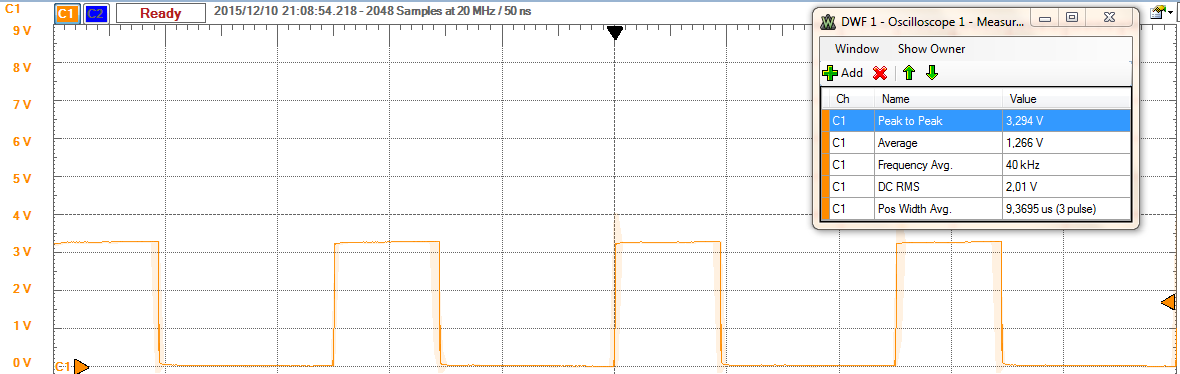
\includegraphics[width=\textwidth* 9/10]{../fig/billeder/steering_pwm_motor_test}
	\caption{Screendump af test af motor PWM}
	\label{fig:steering_pwm_motor_test}
\end{figure}

\begin{figure}[h]
	\centering
	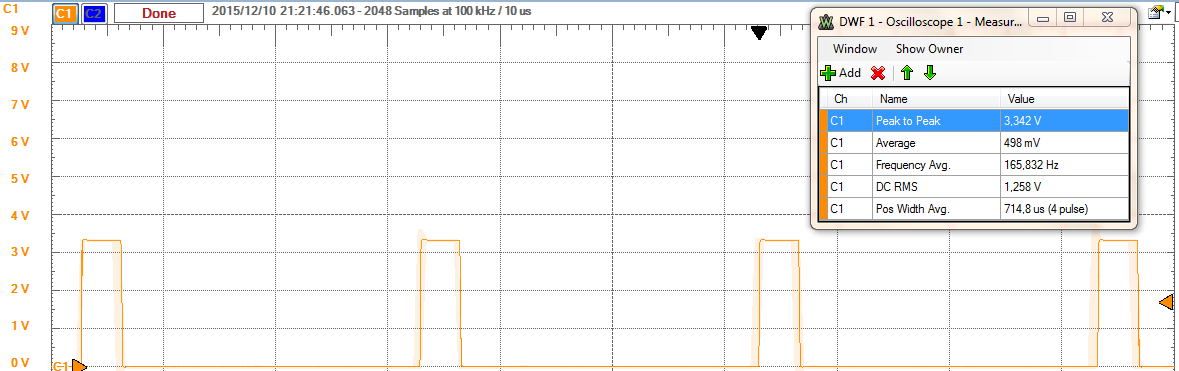
\includegraphics[width=\textwidth* 9/10]{../fig/billeder/steering_pwm_servo_test}
	\caption{Screendump af test af servo PWM}
	\label{fig:steering_pwm_servo_test}
\end{figure}


\subsubsection*{WiringPi} \label{sec:wiringPi_impl}
%lib:wiringpi
For at få et forenklet interface til brugen af Pi'ens GPIO pins (General-purpose input/output) er biblioteket WiringPi \cite{lib:wiringpi_projekt} blevet brugt i implementeringen af Steering klassen. Den er blevet brugt til at sætte frekvensen på PWM signalerne (HW/SW). Hvilke pins der skal bruges til PWM og digitale outputs. Samt opdatere duty cycle af PWM signalerne.
